\documentclass[12pt]{article}%Tamaño de letra y tipo de documento
\usepackage[spanish]{babel}%Importa espanol
\usepackage[utf8]{inputenc}%Importa vocales con tilde
\usepackage{amsmath}%Importamos una fuente para funciones
\usepackage{graphicx}%Importamos la introduccion de imagenes
\usepackage[a4paper,includeheadfoot,margin=2.80cm]{geometry}%Generamos margenes

%Titulo y cosas iniciales
\graphicspath{{Imagenes/}}%Indicamos la direccion de donde coger imagenes

\title{\textbf{\Huge Bienvenido al inicio, creamos un ``¡Hola, mundo!"}}%Atencion a las comillas! textbf lo hace negrita
\date{04/11/2016}
\author{Miguel Bayón\thanks{Dedicado a Pepe Viyuela, por ser calvo}}

\begin{document}

	\maketitle%Insertamos titulo
	\thispagestyle{empty}
	\clearpage%Comenzamos nueva pagina
	
	\tableofcontents%Anadimos indice
	\thispagestyle{empty}
	\clearpage
	
	\setcounter{page}{1}%Ponemos a 1 la nueva pagina, despues del titulo en este caso

	\section{Introduccion}
		¡Hola mundete!
%Procurar dejar una linea en blanco despues de cada parrafo por muy corto que sea para asegurarse de que haga sangrias bien
	\subsection{Vamos viendo}
		¿Qué tal? Este texto está en... ¡Español!
		
		Ampliemos:
		\begin{figure}[h]%h significa: pon la imagen HERE. Con un ! lo fuerza
			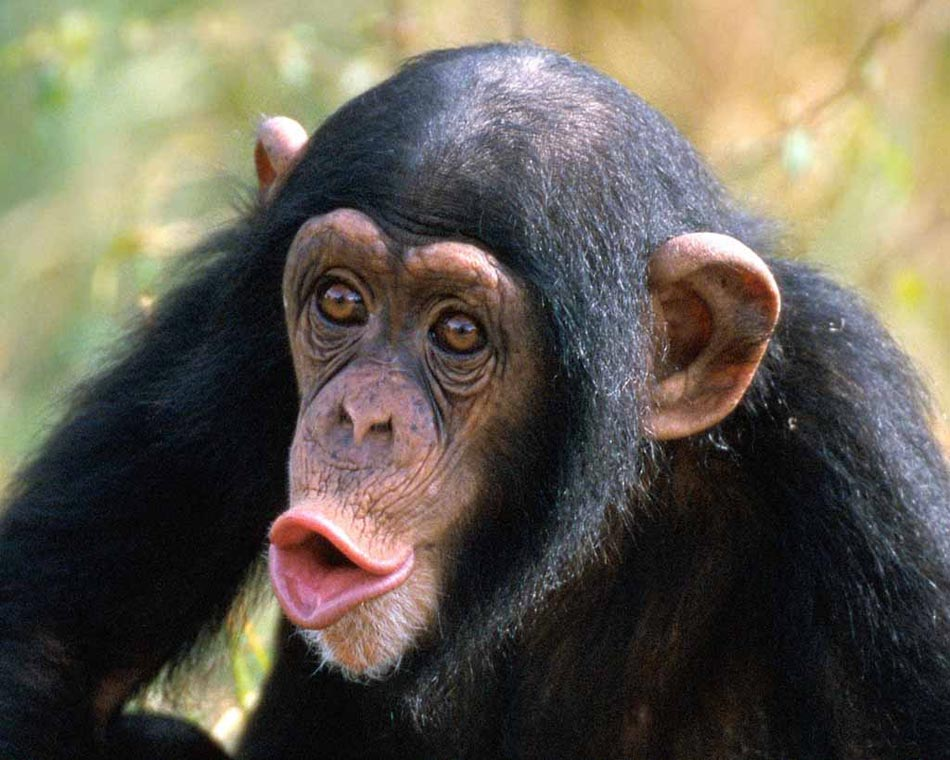
\includegraphics[width=\linewidth]{chimpances}%linewidth ajusta al margen
			\caption{Un monete.}
			\label{fig:monete1}
		\end{figure}
		
		La figura \ref{fig:monete1} nos muestra a un monete.
	\subsubsection{Esto ya es pasarse}
		¿Creando una subsubsección? ¡Venga ya, hombre!

	\section{Volvemos}
		Esto ya es otra cosa. Por ejemplo:
		
	\paragraph{Uno}
		Esto es una cosa
		
	\subparagraph{Dos}
		Esto es la otra
		
	\subsection{Hagamos una ecuacion}
		Para hacerlo, lo escribimos en todo el medio:
		
	\begin{equation}
		f(x)=x^2
	\end{equation}
	
	\subsubsection{La parrafada}
		Pues aquí estamos. Todavía no había escrito más de una línea completa en este texto, así que ahora voy a intentar ocuparme de poner una PARRAFADA en esta subsubsección. Sí, escribo PARRAFADA en mayúsculas porque es el nombre de la subsubsección, como si esto lo hiciera más interesante. A estas alturas ya debería haber pasado de sobra la línea en el texto, así que voy a dejar de escribir. En serio. Y... voy a dejar de escribir... YA.
		
		Supuestamente, y según dicen los tutoriales que voy viendo por Internet, este doble espaciado en el documento .tex debería hacer que comenzase un párrafo nuevo, lo que me preocupa porque nuestro amigo Latex no me hace las sangrías adecuadas.
	
\end{document}